\newcommand{\wormTagResultsAucTable}{
    \begin{table}[H]
        \centering
        \begin{tabular}{|p{2,8cm}||p{2,8cm} p{2,8cm} p{2,8cm}|}
            \hline
            Worm Tag & ALOHA & Joint Embedding & Proposed Model \\
            \hline
            AUC-ROC & 0.616$\pm$0.192 & 0.492$\pm$0.076 & \textBF{0.651$\pm$0.078} \\
            \hline
        \end{tabular}
        \caption{AUC-ROC (Area Under Curve) of the different models for the \textbf{Worm Tag} prediction task. Results were aggregated over \textBF{3} training runs with different weight initializations and minibatch orderings. Best results are shown in \textbf{bold}.} \label{tab:wormTag_auc}
    \end{table}
}

\newcommand{\wormTagResultsAtFprTable}{
    \begin{center}
        \begin{longtable}[c]{|p{3,2cm}||p{1,8cm} p{1,8cm} p{1,8cm} p{1,8cm} p{1,8cm}|}
            \hline
            Worm Tag & \multicolumn{5}{c|}{{FPR}} \\
            & $10^{-5}$ & $10^{-4}$ & $10^{-3}$ & $10^{-2}$ & $10^{-1}$ \\
            \hline
            \endfirsthead

            \caption*{\raggedright ...continued from previous page} \\
            \hline
            Worm Tag & \multicolumn{5}{c|}{\textbf{FPR}} \\
            & $10^{-5}$ & $10^{-4}$ & $10^{-3}$ & $10^{-2}$ & $10^{-1}$ \\
            \hline
            \endhead

            \caption*{\raggedleft ...continued on next page} \\
            \endfoot

            \caption{Mean and standard deviation results (TPR, Accuracy, Recall, Precision and F1-Score) of the different models for the \textbf{Worm Tag} prediction task at different \textbf{FPR}s (\textit{False Positive Rates}). Results were aggregated over \textBF{3} training runs with different weight initializations and minibatch orderings. Best results are shown in \textbf{bold}. Under \textbf{TPR} results are also presented the percentage reduction in mean detection error and in ROC curve standard deviation introduced by the \textit{Proposed Model} with respect to both \textit{ALOHA} model and \textit{Joint Embedding}.} \label{tab:wormTag_results_at_fpr} \\
            \endlastfoot

            \multicolumn{6}{|c|}{\textbf{TPR}} \\
            \hline
            ALOHA & 0.000$\pm$0.000 & 0.000$\pm$0.000 & 0.016$\pm$0.010 & 0.069$\pm$0.024 & 0.202$\pm$0.115 \\
            Joint Embedding & \textBF{0.083$\pm$0.060} & \textBF{0.083$\pm$0.060} & 0.087$\pm$0.057 & 0.109$\pm$0.064 & 0.214$\pm$0.018 \\
            Proposed Model & 0.048$\pm$0.008 & 0.048$\pm$0.008 & \textBF{0.100$\pm$0.071} & \textBF{0.129$\pm$0.064} & \textBF{0.432$\pm$0.128} \\
            \hline
            Error Reduction wrt \newline ALOHA & 4.8\% & 4.8\% & 8.5\% & 6.4\% & 28.8\% \\
            Error Reduction wrt \newline Joint Embedding & -3.8\% & -3.8\% & 1.4\% & 2.2\% & 27.7\% \\
            \hline
            Std Reduction wrt \newline ALOHA & 0.0\% & 0.0\% & -610.0\% & -166.7\% & -11.3\% \\
            Std Reduction wrt \newline Joint Embedding & 86.7\% & 86.7\% & -24.6\% & 0.0\% & -611.1\% \\
            \hline
            \multicolumn{6}{|c|}{\textbf{Accuracy}} \\
            \hline
            ALOHA & 0.895$\pm$0.000 & 0.895$\pm$0.000 & 0.896$\pm$0.001 & 0.894$\pm$0.002 & 0.828$\pm$0.013 \\
            Joint Embedding & \textBF{0.904$\pm$0.006} & \textBF{0.904$\pm$0.006} & 0.904$\pm$0.006 & 0.898$\pm$0.007 & 0.831$\pm$0.004 \\
            Proposed Model & 0.900$\pm$0.001 & 0.900$\pm$0.001 & \textBF{0.905$\pm$0.007} & \textBF{0.900$\pm$0.007} & \textBF{0.852$\pm$0.014} \\
            \hline
            \multicolumn{6}{|c|}{\textbf{Recall}} \\
            \hline
            ALOHA & 0.000$\pm$0.000 & 0.000$\pm$0.000 & 0.016$\pm$0.010 & 0.069$\pm$0.024 & 0.202$\pm$0.115 \\
            Joint Embedding & \textBF{0.083$\pm$0.060} & \textBF{0.083$\pm$0.060} & 0.087$\pm$0.057 & 0.109$\pm$0.064 & 0.214$\pm$0.018 \\
            Proposed Model & 0.048$\pm$0.008 & 0.048$\pm$0.008 & \textBF{0.100$\pm$0.071} & \textBF{0.129$\pm$0.064} & \textBF{0.432$\pm$0.128} \\
            \hline
            \multicolumn{6}{|c|}{\textbf{Precision}} \\
            \hline
            ALOHA & \textBF{1.000$\pm$0.000} & \textBF{1.000$\pm$0.000} & 0.637$\pm$0.215 & 0.438$\pm$0.098 & 0.182$\pm$0.098 \\
            Joint Embedding & \textBF{1.000$\pm$0.000} & \textBF{1.000$\pm$0.000} & \textBF{0.958$\pm$0.059} & 0.529$\pm$0.127 & 0.205$\pm$0.010 \\
            Proposed Model & \textBF{1.000$\pm$0.000} & \textBF{1.000$\pm$0.000} & 0.950$\pm$0.046 & \textBF{0.588$\pm$0.107} & \textBF{0.330$\pm$0.072} \\
            \hline
            \multicolumn{6}{|c|}{\textbf{F1 Score}} \\
            \hline
            ALOHA & 0.000$\pm$0.000 & 0.000$\pm$0.000 & 0.030$\pm$0.018 & 0.119$\pm$0.040 & 0.191$\pm$0.106 \\
            Joint Embedding & \textBF{0.148$\pm$0.098} & \textBF{0.148$\pm$0.098} & 0.155$\pm$0.094 & 0.179$\pm$0.094 & 0.209$\pm$0.013 \\
            Proposed Model & 0.092$\pm$0.015 & 0.092$\pm$0.015 & \textBF{0.174$\pm$0.112} & \textBF{0.208$\pm$0.091} & \textBF{0.374$\pm$0.094} \\
            \hline
        \end{longtable}
    \end{center}
}

\newcommand{\wormTagResultsSummaryTable}{
    \begin{table}[H]
        \centering
        \begin{tabular}{|p{3,2cm}||p{1,8cm} p{1,8cm} p{1,8cm} p{1,8cm} p{1,8cm}|}
            \hline
            \multicolumn{6}{|c|}{Worm Tag (at FPR $=1\%$)} \\
            \hline
            Model & TPR & Accuracy & Precision & Recall & F1 score \\
            \hline
            ALOHA & 0.069$\pm$0.024 & 0.894$\pm$0.002 & 0.438$\pm$0.098 & 0.069$\pm$0.024 & 0.119$\pm$0.040 \\
            Joint Embedding & 0.109$\pm$0.064 & 0.898$\pm$0.007 & 0.529$\pm$0.127 & 0.109$\pm$0.064 & 0.179$\pm$0.094 \\
            Proposed Model & \textBF{0.129$\pm$0.064} & \textBF{0.900$\pm$0.007} & \textBF{0.588$\pm$0.107} & \textBF{0.129$\pm$0.064} & \textBF{0.208$\pm$0.091} \\
            \hline
        \end{tabular}
        \caption{Summary of the mean and standard deviation results of the different models for the \textbf{Worm Tag} prediction task at \textbf{FPR} $=1\%$. Results were aggregated over \textBF{3} training runs with different weight initializations and minibatch orderings. Best results are shown in \textbf{bold}.} \label{tab:wormTag_result_summary}
    \end{table}
}

\newcommand{\wormTagRocAloha}{
    \begin{figure}[H]
        \vspace*{-0.5cm}
        \centering
        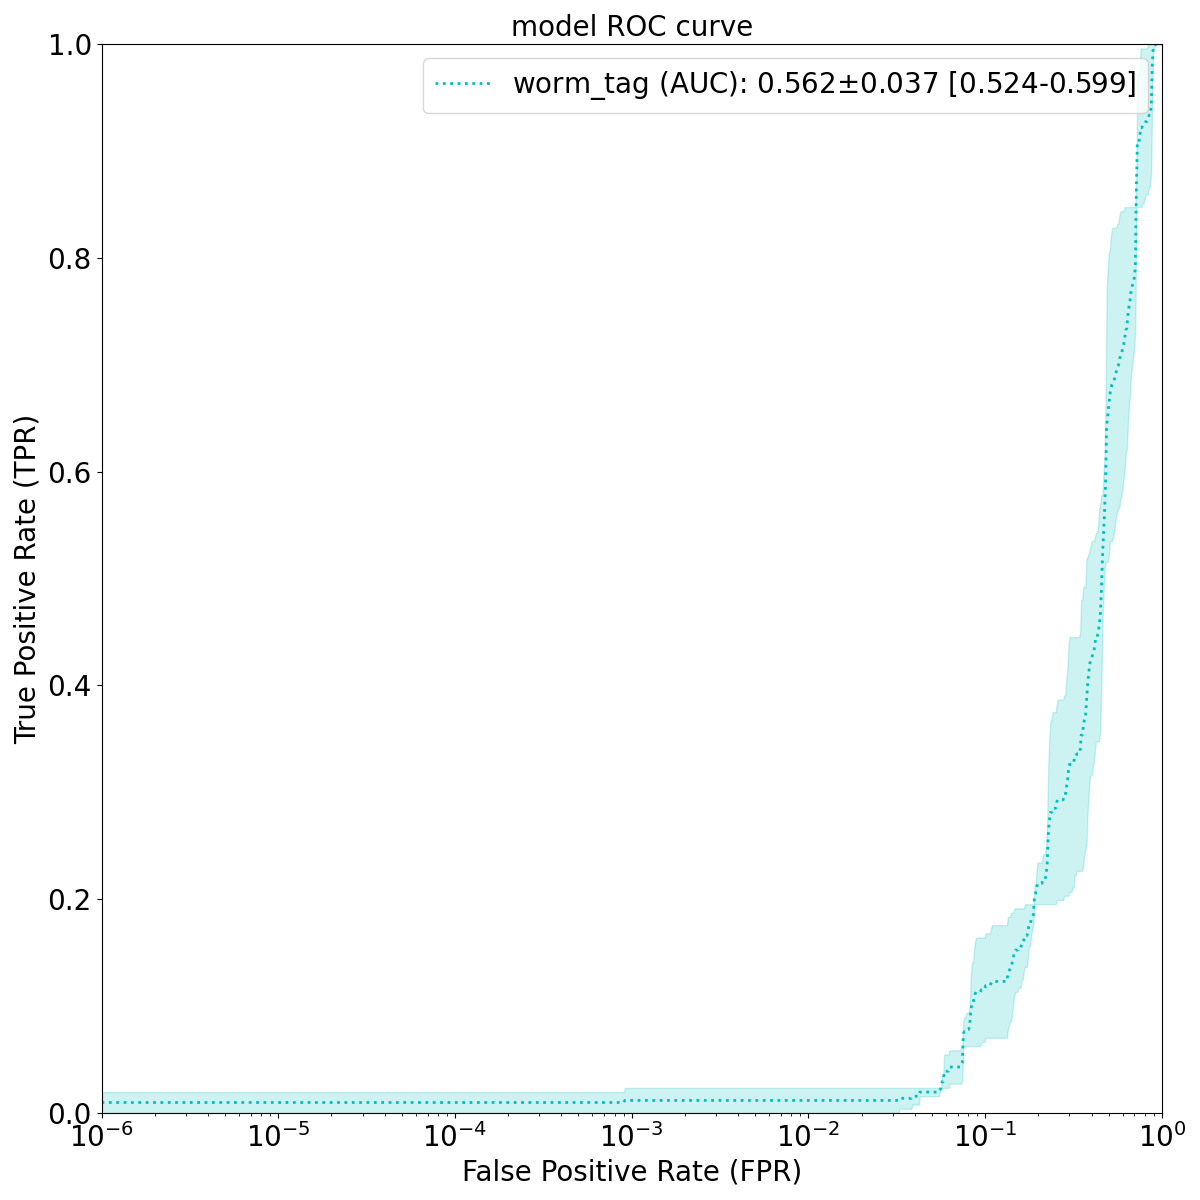
\includegraphics[width=0.6\textwidth]{./results/worm_tag_roc_aloha.png}
        \vspace*{-0.2cm}
        \caption{ROC curve and AUC statistics of \textBF{ALOHA} model for the \textbf{Worm Tag}. The line represents the \textit{mean} TPR at a given FPR, while the shaded region represents the \textit{standard deviation}. Statistics were computed over \textBF{3} training runs, each with random parameter initialization.}
        \label{fig:wormTagRocAloha}
    \end{figure}
}

\newcommand{\wormTagRocJointEmbedding}{
    \begin{figure}[H]
        \vspace*{-0.5cm}
        \centering
        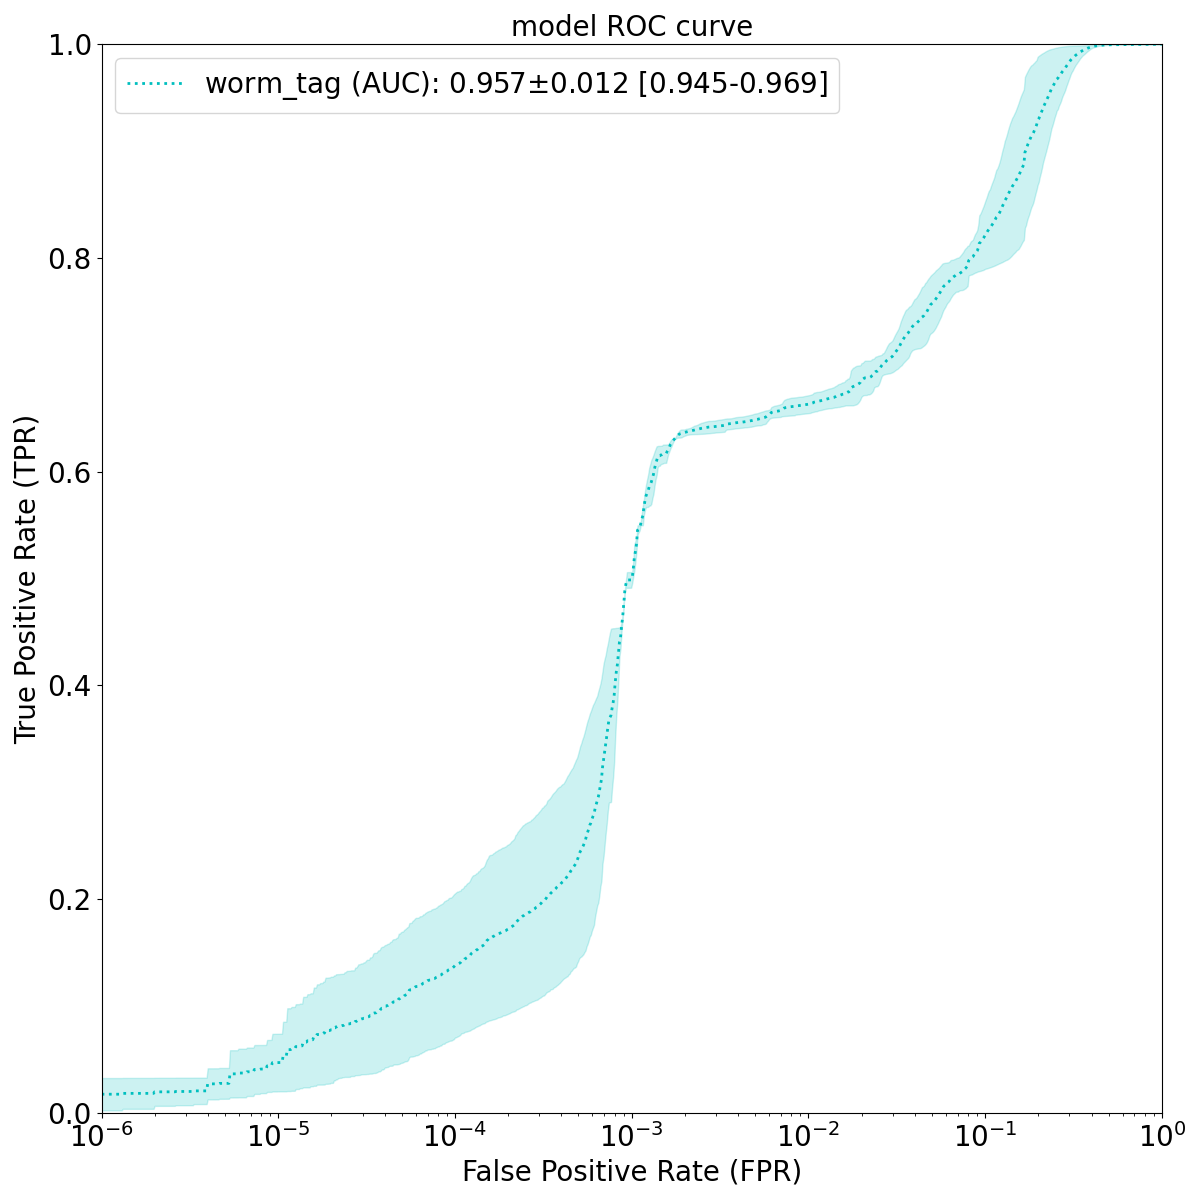
\includegraphics[width=0.6\textwidth]{./results/worm_tag_roc_jointEmbedding.png}
        \vspace*{-0.2cm}
        \caption{ROC curve and AUC statistics of \textBF{Joint Embedding} model for the \textbf{Worm Tag}. The line represents the \textit{mean} TPR at a given FPR, while the shaded region represents the \textit{standard deviation}. Statistics were computed over \textBF{3} training runs, each with random parameter initialization.}
        \label{fig:wormTagRocJointEmbedding}
    \end{figure}
}

\newcommand{\wormTagRocProposedMethod}{
    \begin{figure}[H]
        \vspace*{-0.5cm}
        \centering
        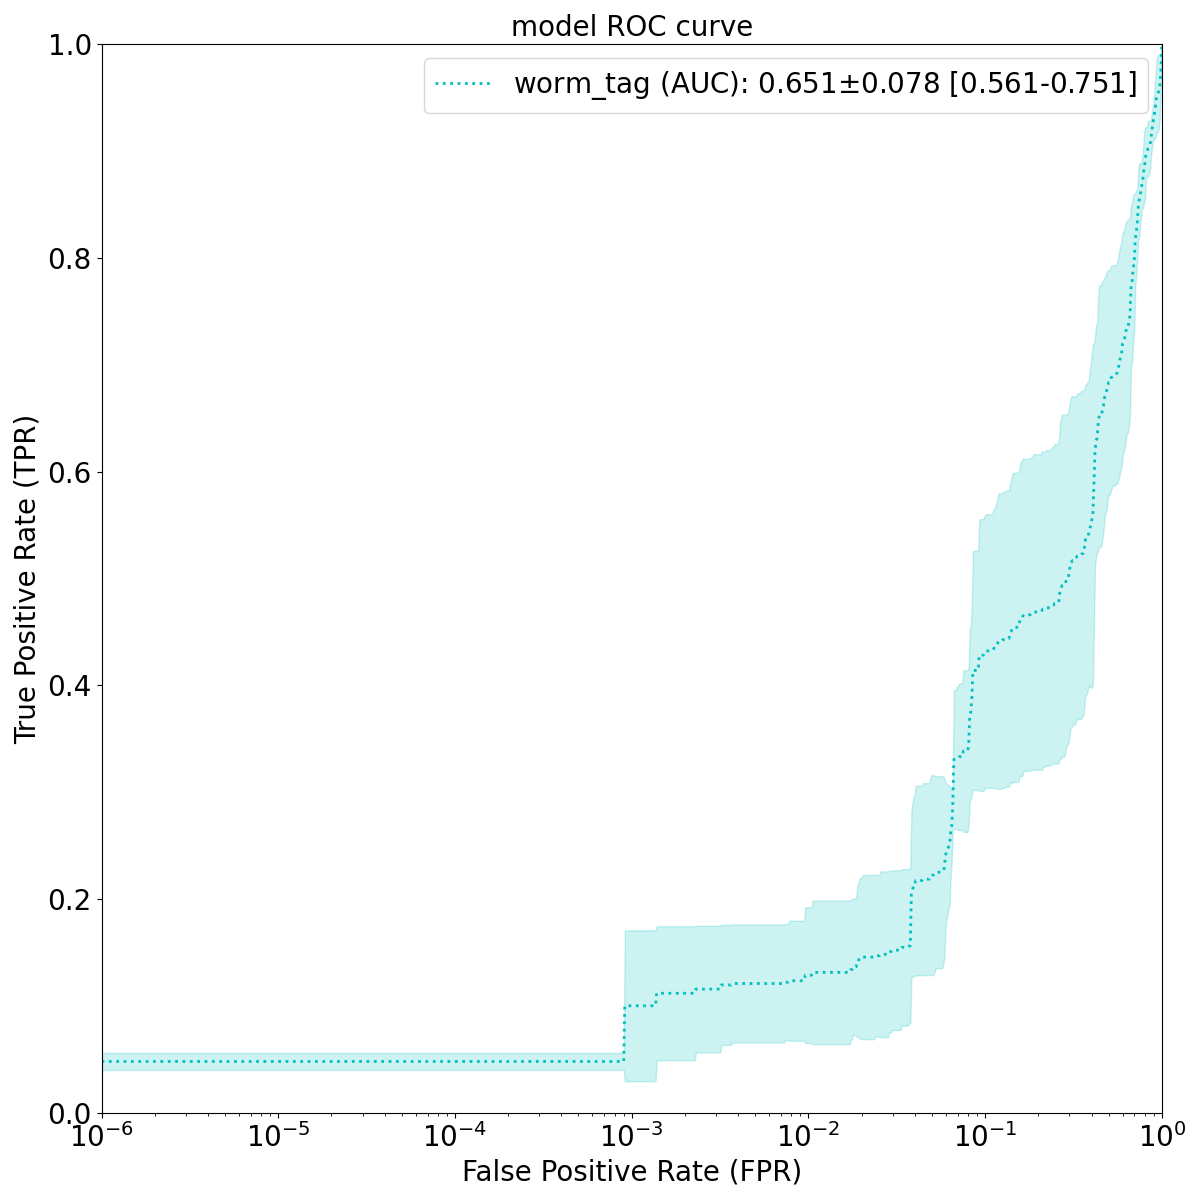
\includegraphics[width=0.6\textwidth]{./results/worm_tag_roc_proposedModel.png}
        \vspace*{-0.2cm}
        \caption{ROC curve and AUC statistics of \textBF{Proposed Model} for the \textbf{Worm Tag}. The line represents the \textit{mean} TPR at a given FPR, while the shaded region represents the \textit{standard deviation}. Statistics were computed over \textBF{3} training runs, each with random parameter initialization.}
        \label{fig:wormTagRocProposedModel}
    \end{figure}
}
